\subsection{Opgave 28}

Funktionen f er bestemt ved

\begin{align*}
    f(x) = -2\cdot x + 4
\end{align*}

Forklar hvilken betydning tallene -2 og 4 har for grafens udseende.

\ans

Hvis vi sammenligner funktionen $f(x) = -2\cdot x + 4$
for forskellige funktioners forskrifter kan vi se at det er en lineær funktion 
da den matcher med den generelle forskrift for en lineær funktion
$f(x) = a\cdot x + b$.

Vi ved at a værdien for en lineær funktion er dens hældning, dvs når vi går en ud af x aksen, går funktionen hældningen
op eller ned. b værdien er funktionens skæring med y aksen.

Det vil sige at de -2 er hældningen for funktionen $f(x)$ og hver gang vi går 1 ud af x aksen
går funktionen 2 ned.

Tallet 4 fortæller at funktionen $f(x)$ skærer y aksen i $y = 4$.

Nedenfor er funktionen $f(x)$ indtegnet i GeoGebra hvor hældningen på -2 og skæringen med y aksen i 
$y = 4$ er markeret.

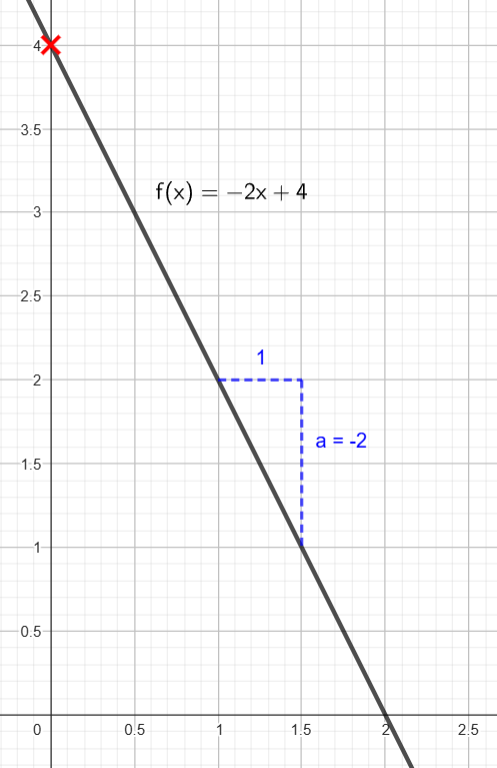
\includegraphics[width=6cm]{Opgave_21-30/Opgave_28/28.png}